\documentclass[border=4pt]{standalone}
\usepackage{tikz}
\usetikzlibrary{arrows.meta,positioning,shapes.geometric,topaths}
\tikzset{
  stage/.style={draw,rounded corners=2pt,minimum width=24mm,minimum height=9mm,align=center},
  decision/.style={diamond,draw,aspect=2,inner sep=1pt,align=center},
  hv route/.style={to path={-| (\tikztotarget) \tikztonodes}},
  vh route/.style={to path={|- (\tikztotarget) \tikztonodes}}
}
\begin{document}
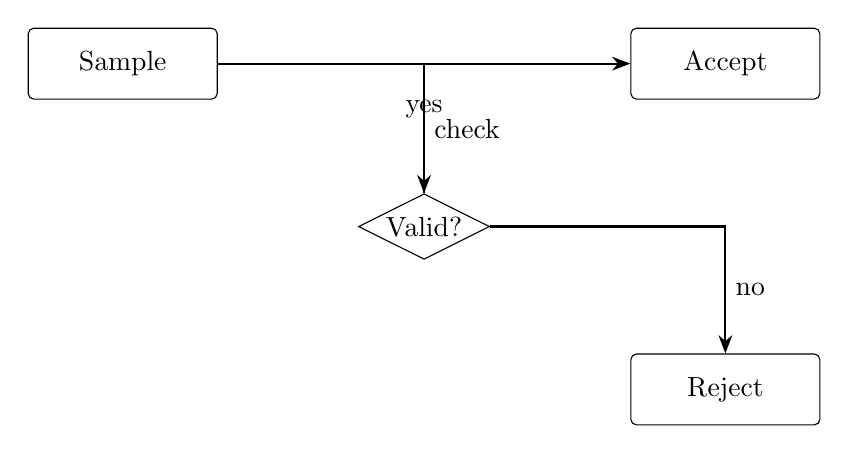
\begin{tikzpicture}[node distance=14mm and 22mm,>=Stealth]
  \node[stage] (sample) {Sample};
  \node[decision,below right=of sample] (valid) {Valid?};
  \node[stage,above right=of valid] (accept) {Accept};
  \node[stage,below right=of valid] (reject) {Reject};
  \draw[->,thick,hv route] (sample) to node[near end,right] {check} (valid);
  \draw[->,thick,vh route] (valid) to node[near start,above] {yes} (accept);
  \draw[->,thick,hv route] (valid) to node[near end,right] {no} (reject);
\end{tikzpicture}
\end{document}
